\documentclass{article}

\usepackage{amsthm}
	\newtheorem*{definition}{Definition}
	\newtheorem*{theorem}{Theorem}
	\newtheorem*{lemma}{Lemma}
\usepackage{amsmath}
\usepackage{amsfonts}
\usepackage{amssymb}
\usepackage[margin=1in]{geometry}
\usepackage{hyperref}
\usepackage{tikz}
	\usetikzlibrary{cd}
	\usetikzlibrary{patterns}
	\usetikzlibrary{decorations.markings}
	
\DeclareMathOperator{\Tor}{Tor}
\newcommand{\Z}{\mathbb{Z}}
\renewcommand{\theequation}{\roman{equation}}

\title{\href{https://math.umn.edu/sites/math.umn.edu/files/exams/mantops18.pdf}{Spring 2018 Manifolds and Topology Preliminary Exam}}
\author{University of Minnesota}
\date{}
\begin{document}
\maketitle

\section*{Part A}
\begin{enumerate}
	\item Define what it means for two continuous paths $\alpha, \beta: [0,1] \rightarrow X$, both starting at the same point $p$ and ending at the same point $q$, to be homotopic. Define the fundamental group $\pi_1 (X, p)$ as a set.
	
	\begin{definition}
		Two paths $\alpha, \beta$ as given above are said to be homotopic (written $\alpha \sim \beta$),
		if there exists a continuous map $H(s,t): [0,1]^2 \rightarrow X$ such that $\alpha(t) = H(0,t)$ and $\beta(t) = H(1,t)$.
	\end{definition}
	
	\begin{definition}
		Note that the relation $\sim$ defines an equivalence relation on all continuous paths sharing a common starting and ending point. 
		If a continous path starts and ends at the same point $p$, we call it a loop in $X$ with basepoint $p$.
		Let $\mathcal{L}_p = \{ \text{loops in $X$ with basepoint $p$} \}$.
		Then as a set, $\pi_1(X,p) = \mathcal{L}_p / \sim$ is the set of equivalence classes of $\mathcal{L}_p$ under $\sim$. 
	\end{definition}
	
	\item Suppose $X$ is a space. Define what it means for two covering maps $p: Y \rightarrow X$ and $q: Z \rightarrow X$ to be isomorphic.
	
	\begin{definition}
		Two covering maps $p:Y \rightarrow X$, $q:Z \rightarrow X$ are isomorphic if $f:Y \rightarrow Z$ is a homeomorphism and the following diagram commutes
		
		\begin{center}
		\begin{tikzcd}
			Y \arrow[rr,"f"] \arrow[rd,"p"'] & &Z \arrow{ld}{q} \\
			& X&
		\end{tikzcd}
		\end{center}
		
	\end{definition}
	
	\item Suppose $p$ is a point in the space $X$ and $\alpha$ is a loop in $X$ starting and ending at a point $p$. If $c$ is the constant loop at $p$, show explicitly that the concatenated loop $\alpha * c$ is homotopic to $\alpha$.
	
	\begin{proof}
		Recall that concatenation of loops $\gamma_1, \gamma_2$ is given as
		\[ \gamma_1 * \gamma_2 = \begin{cases} \gamma_1(2t) & t \in [0,1/2] \\ \gamma_2(2t-1) & t \in (1/2,1]\end{cases},\]
		so 
		\[ \alpha * c = \begin{cases} \alpha(2t) & t \in [0,1/2] \\ p & t \in (1/2,1].\end{cases}\]
		
		Define 
		\[H(s,t) = \begin{cases} 
					\alpha(\frac{2t}{1+s}) & t \in [0,\frac{s+1}{2}] \\
			     		c & t \in (\frac{s+1}{2},1].
			      \end{cases}\]
		
		Note that $H(0,t) = \alpha * c$ and $H(1,t) = \alpha$ and $H(s,t)$ is continuous in $s$ since $\frac{2}{1+s}$ is continuous. 
	\end{proof}
	
	%\item Prove that a covering map $Y \rightarrow X$ of path-connected spaces and a point $p \in X$ determine a well defined \textit{conjugacy class} of subgroup $H$ of $\pi_1(X,p)$.
	
	\setcounter{enumi}{4}
	\item Suppose $X$ is a space with open subsets $U$ and $V$ such that $X$ is the union $U \cup V$, both $U,V$ are simply-connected, and $H_1(U \cap V) \neq 0$. Show that $H_2(X)$ is nontrivial.
	
	\begin{proof}
		We know that given $U,V$ as above, we have the Mayer-Vietoris long exact sequence:	
		
		\begin{center}
		\begin{tikzcd}
			\cdots \arrow[r] %& H_2(U) \otimes H_2(V) \arrow[r] 
			& H_2(X) \arrow[r] & H_1(U \cap V) \arrow[r] & H_1(U) \otimes H_1(V) \arrow[r] &\cdots 
		\end{tikzcd}
		\end{center}
		
		Since $U,V$ are simply connected, they have trivial $pi_1$. 
		$H_1$ is the abelianization of $\pi_1$, and so since the trivial group is abelian, we have
		$H_1(U) \otimes H_1(V) = 0 \otimes 0 \cong 0$.
		
		We are also given that $H_1(U \cap V) \neq 0$.
		
		Thus, the map $H_1(U \cap V) \rightarrow 0$ is the zero map. Then exactness of the sequence tells us that
		 ${H_2(X) \rightarrow H_1(U \cap V) \neq 0}$ is a surjection. This shows that $H_2(X)$ is nontrivial, since the map
		 ${0 \rightarrow H_1(U\cap V) \neq 0}$ can never be a surjection.
	\end{proof}
	
	\setcounter{enumi}{7}
	
	\item Let $M$ be the M\"obius band
	\[ [0,1]^2 / \{(x,0) \sim (1-x,1)\}\]
	with boundary $\partial M$. Show that there does not exist a continuous retraction $r:M \rightarrow \partial M$.
	
	\begin{proof}{(From \href{https://math.stackexchange.com/questions/202447/retraction-of-the-m\%C3\%B6bius-strip-to-its-boundary}{StackExchange})}
	Suppose that $\pi_1(\partial M) = \langle \alpha \rangle$ and $\pi_1(M) = \langle \beta \rangle$. The picture
	
	\begin{center}
	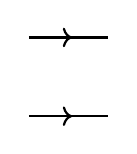
\begin{tikzpicture}[thick,decoration={
		markings,
		mark=at position 0.55 with {\arrow{>}}}
		] 
	\draw[postaction={decorate}] (0,0)--(1,0);
	%\draw[postaction={decorate}] (1,0)--(1,1);
	\draw[postaction={decorate}] (0,1)--(1,1);
	%\draw[postaction={decorate}] (0,1)--(0,0);
	\end{tikzpicture}
	\hspace{1in}
	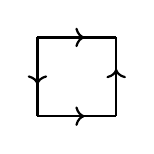
\begin{tikzpicture}[thick,decoration={
		markings,
		mark=at position 0.6 with {\arrow{>}}}
		] 
	\draw[postaction={decorate}] (0,0)--(1,0);
	\draw[postaction={decorate}] (1,0)--(1,1);
	\draw[postaction={decorate}] (0,1)--(1,1);
	\draw[postaction={decorate}] (0,1)--(0,0);
	\end{tikzpicture}
	\end{center}
	
	shows that the inclusion $\iota: \partial M \rightarrow M$ induces the homomorphism $\iota_* : \pi_1(\partial M) \rightarrow \pi_1(M),$
	where $\iota_*(\alpha) = \beta^2$, since the boundary must be traversed twice to have a closed loop.
	
	If there were a retraction $r: M \rightarrow \partial M$, then the induced homomorphism $r_*$ on fundamental groups would satisfy $r_*\circ \iota_* (\alpha) = \alpha$. But $\iota_*(\alpha) = \beta^2$, so then $r_*(\beta^2) = r_*(\beta)^2 = \alpha$, or $r_*(\beta) = \sqrt{\alpha} \not \in \pi_1(\partial M)$.
	\end{proof}
	
	\item Suppose $X$ is a (connected, locally contractible) space whose fundamental group is the group $\mathbb{Z}/2 \times \mathbb{Z}/4.$
	How many isomorphism classes of covering maps $Y \rightarrow X$ are there with $Y$ path-connected.
	
	\begin{proof}
		Isomorphism classes of path connected covering spaces are in bijection with conjugacy classes of subgroups of the fundamental group. 
		When the fundamental group is abelian, the conjugacy classes of subgroups are simply 
		the subgroups (since $ghg^{-1} = gg^{-1} h=h$) of the group. 
		Note that $\mathbb{Z}/2 \times \mathbb{Z}/4$ is abelian, and has $8$ subgroups.
		
		Namely, Goursat's lemma tells us the subgroups are in bijection with 5-tuples $(G_1, G_2, H_1, H_2, \varphi)$
		where $G_1 \trianglelefteq G_2 \leq Z/2$ and $H_1 \trianglelefteq H_2 \leq \mathbb{Z}/4$, and $\varphi: G_2/G_1 \rightarrow H_2/H_1$
		is an isomorphism. The possible pairs of $G_1,G_2$ are:
		\[ ( \{0\},\{0\}), (\{0\}, Z/2), (\Z/2, \Z/2)\]
		yielding quotients
		\[ 0 \cong 0/0, \Z/2 \cong \Z/2 / 0, 0 \cong \Z/2 / \Z/2\]
		and the possible pairs $H_1,H_2$ are:
		\[ ( \{0\},\{0\}), (\{0\}, \Z/2), (\{0\}, \Z/4), (\Z/2, \Z/2),(\Z/2, \Z/4), (\Z/4, \Z/4) \]
		which yield quotients:
		\[ 0, \Z/2, \Z/4, 0, \Z/2, 0 \].
		
		There are 6 different 4-tuples of quotients who yield the trivial group. The only isomorphism of the trivial group is the trivial map, so
		these contribute +6 to our count of of subgroups.
		%
		There are 2 different 4-tuples of quotients who yield the group $\Z/2$.
		Similarly, there is only one isomorphism from $\Z/2$ to itself.
		Thus, there are 8 subgroups of $\Z/2\times \Z/4$ and so there are 8 isomorphism classes of covering maps $Y \rightarrow X$ 
		with $Y$ being path connected.
		
		\emph{Note:} 6 of the subgroups are of the form $G \times H$ where $G \leq \Z/2$ and $H \leq \Z/4$.
		The two remaining subgrops are 
		
		\[ \langle (1,0) + (1,3) \rangle \]
	\end{proof}
	
	\href{https://math.stackexchange.com/questions/666840/what-are-the-subgroups-of-bbbz-2-times-bbbz-4}{Alternate proof.}
\end{enumerate}

\section*{Part B}
\begin{enumerate}
	\item	 
\end{enumerate}

\end{document}